\section{模型的建立与求解}

\subsection{问题1-1:结合解析几何,建立被动接受信号无人机的定位模型}

针对于问题(1),需要建立坐标系确定各无人机的位置,并引入相关数学模型使各无人机涉及到的参量具有数学关系,进一步加强对定位模型合理准确的建立。分析题目可知,可以用的坐标系有极坐标和空间直角坐标。对极坐标而言,当题目已确定无人机群处于同一个高度平面,所以可以引入极径$\rho$与极角$\alpha$两个因变量。对于空间直角坐标而言,至少存在两个以上的因变量,依题意对于无人机群控制在同一高度则可令$z=\alpha$,其中$x$与$y$为确定单无人机的具体位置。本文建立了基于同高度且按圆周均匀分布的间接式立体定位模型,通过对单无人机逐个编队,使之形成均匀圆周分布的定位模型。

\begin{figure}[h]
    \centering
    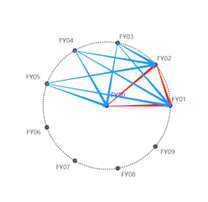
\includegraphics{res/AerialView.png}
    \caption{空间立体鸟瞰图}
\end{figure}

\textbf{模型一的建立——空间立体直角坐标定位模型}

依题意在空间直角坐标系中 是确定的,假定引入一参照物观测站(相对于原点 ),定位模型处于空间直角坐标系中,则无人机所到目标位置的真实坐标为 ,无人机观测站的坐标为 。各无人机到目标之间的距离为
 (1-1)

令

\begin{equation}
\begin{cases}
    r^2 = x_t^2 + y_t^2 + z_t^2   \\
    r^2_i = x_i^2 + y_i^2 + z_i^2 \\
\end{cases}
\label{e5-081538}
\end{equation}

在\eqref{e5-081537}式中,$r$为目标位置与坐标原点之间的距离,对\eqref{e5-081537}式平方联立\eqref{e5-081538}式可以得到\cite{weilian*feileGailulunjiqiyingyong}

\begin{equation}
\rho^2_i - r^2_i - r
= -2(x_ix_t + y_iy_t + z_iz_t)
\label{e5-081539}
\end{equation}

既有:

\begin{equation}
    \begin{cases}
        \rho_1^2 - r_1^2 - r^2 = -2(x_1x_t + y_1y_t + z_1z_t)   \\
        \rho_2^2 - r_2^2 - r^2 = -2(x_2x_t + y_2y_t + z_2z_t)   \\
        \rho_3^2 - r_3^2 - r^2 = -2(x_3x_t + y_3y_t + z_3z_5)   \\ 
    \end{cases}
\end{equation}

既有传统定位方程如\eqref{e5-081539}式所示,将其写成为矩阵形式有:

\begin{equation}
    A_1x_t = B_1
\end{equation}

其中:

\begin{equation}
    B_1=
    \left[
    \begin{matrix}
        \rho_1^2 - r_1^2 - r^2 \\
        \rho_2^2 - r_2^2 - r^2 \\
        \rho_3^2 - r_3^2 - r^2 \\
    \end{matrix}
    \right]
    A_1=
    \left[
    \begin{matrix}
        -2x_1 - 2y_1 - 2z_1 \\
        -2x_2 - 2y_2 - 2z_2 \\
        -2x_3 - 2y_3 - 2z_3 \\
    \end{matrix}
    \right]
    \notag
\end{equation}

计算上式,目标大致为$x_0$为:

\begin{equation}
    x_0 = A_1^{-1}B_1
    \label{e5-081704}
\end{equation}

引入偏差$\varepsilon_{\rho i}$构建定位方程为:

\begin{equation}
    \rho_i = \|x_i - x_t\| + \varepsilon_{\rho i}, i=1,2,3
\end{equation}

令$\varepsilon_{\rho i}~N(0, \sigma_\rho^2)$,将上式右边于$x_0$处进行泰勒展开并忽略最高项得到:

\begin{equation}
    \rho_i = \|x_i-x_0\|
    - \frac{(x_i-x_0)(x_t-x_0)}{\|x_i-x_0\|}
    - \frac{(y_i-y_0)(y_t-y_0)}{\|x_i-x_0\|}
    - \frac{(z_i-z_0)(z_t-z_0)}{\|x_i-x_0\|}
    + \varepsilon_{\rho i}
\end{equation}

得到初步定位方程,写成矩阵形式如下:

\begin{equation}
    Ay=B
    \label{e5-matrix}
\end{equation}

在\eqref{e5-matrix}式中:

\begin{equation}
    A=
    \left[
    \begin{matrix}
        \frac{x_1-x_0}{\rho'_1} & \frac{y_1-y_0}{\rho'_1} & \frac{z_1-z_0}{\rho'_1} \\

        \frac{x_2-x_0}{\rho'_2} & \frac{y_2-y_0}{\rho'_2} & \frac{z_2-z_0}{\rho'_2} \\
        
        \frac{x_3-x_0}{\rho'_3} & \frac{y_3-y_0}{\rho'_3} & \frac{z_3-z_0}{\rho'_3} \\
    \end{matrix}
    \right]
    y=
    \left[
        \begin{matrix}
            x_t - x_0   \\
            y_t - y_0   \\
            z_t - z_0   \\
        \end{matrix}
    \right]
\end{equation}

且

\begin{equation}
    B=
    \left[
        \begin{matrix}
            \rho'_1-\rho_1+\varepsilon_{\rho1} \\
            \rho'_2-\rho_2+\varepsilon_{\rho2} \\
            \rho'_3-\rho_3+\varepsilon_{\rho3} \\
        \end{matrix}
    \right]
    \|x_i - x_0\| = \rho'_i
\end{equation}

综上可解得初步定位方程得解为:

\begin{equation}
    y=A^{-1}B
\end{equation}

令无人机观测站站址偏差为$\Delta x_i$,且满足$\Delta x_i~N(0,\sigma_i^2)$,引入方程\eqref{e5-081704}进而得到最终得定位方程为:

\begin{equation}
\left[
    \begin{matrix}
        \frac{x_i-x_0}{\rho'_i} - a_i\Delta x_i     &   \frac{y_i-y_0}{\rho'_i} - b_i\Delta x_i     &   \frac{z_i-z_0}{\rho'_i} - c_i\Delta x_i \\
    \end{matrix}
\right]
\left[
    \begin{matrix}
        x_t - x_0   \\
        y_t - y_0   \\
        z_t - z_0   \\
    \end{matrix}
\right]
=
\rho'_i - d\Delta x_i - \rho_i + \varepsilon_{\rho i}
\end{equation}

……

综上联立上式得表达式定位解为:

\begin{equation}
    y_{Tu}=
    \left (
        A^TH_y^{-2}A
        +
        \left (
            \frac{1}{2}\min\frac{E{c_{2i^2}}}{c_{li}^2\mu_i} +
            \frac{1}{2}\max\frac{E{c_{2i}^2}}{c_{li}^2\mu_i}
        \right )
    \right )
\end{equation}

\textbf{模型特征值检验}:为验证所提定位模型得有效性及适应性,本题对题设的假设条件进行带入检验,依题意即得$\alpha=40$,半径为常数$\rho$,既有$x=\rho\cos\alpha, y=\rho\sin\alpha,z=\theta$,$\theta$为常数。对假设检验数据有下:

\begin{table}[htp!]
    \centering
    \caption{空间坐标}
    \begin{tabular}{cccc}
        \hline
        编号&   坐标变换(极→直)&   编号&   坐标变换(极→直)  \\
        \hline

        0&  (0, 0)→(0, 0, 0)&  5& (10, 160)→(-9.4, 3.42, 0)   \\
        1&  (10, 0)→(10, 0, 0)&    6&  (10, 200)→(-9.4, -3.42, 0)    \\
        2& (10, 40)→(7.66, 6.43, 0)&    7&  (10, 240)→(-5, -8,66, 0)    \\
        3& (10, 80)→(1.74, 9.85, 0)&   8&  (10, 280)→(1.74, -9.85, 0)  \\
        4&  (10, 120)→(-5, 8.66, 0)&    9&  (10, 320)→(7.66, -6.43, 0)  \\

        \hline
    \end{tabular}
\end{table}

\textbf{Step 1:}插入符合题设数据
对符合第一小问的题设加入假定数据进行数据预处理,分别对编号00~09的十架无人机插入已知假定的空间坐标;

\textbf{Step2:}对空间坐标可用极坐标调节简化
对极坐标设置两个参数进行极坐标转换,即极坐标依据空间坐标而成三角函数的数学关系进行变换,设置理想的定位模型以便两坐标的参照对比;\cite{wangnengbinShujukuxitongjiaocheng}

\textbf{Step3:}导入相应数据进行模型检验。

利用$Origin$软件对假定数据建立空间立体检验图,并将上式定位解拟合函数,呈现结果如下。若与图形相符,则该模型可视为定位模型。

综上通过对数据处理,基于定位模型的定位一般方程的建立求解,并且引入符合题意的假设数值进行检验,控制高度一致使得无人机群在同一平面得到如下图所示的空间立体模型图:


\begin{figure}
    \centering
    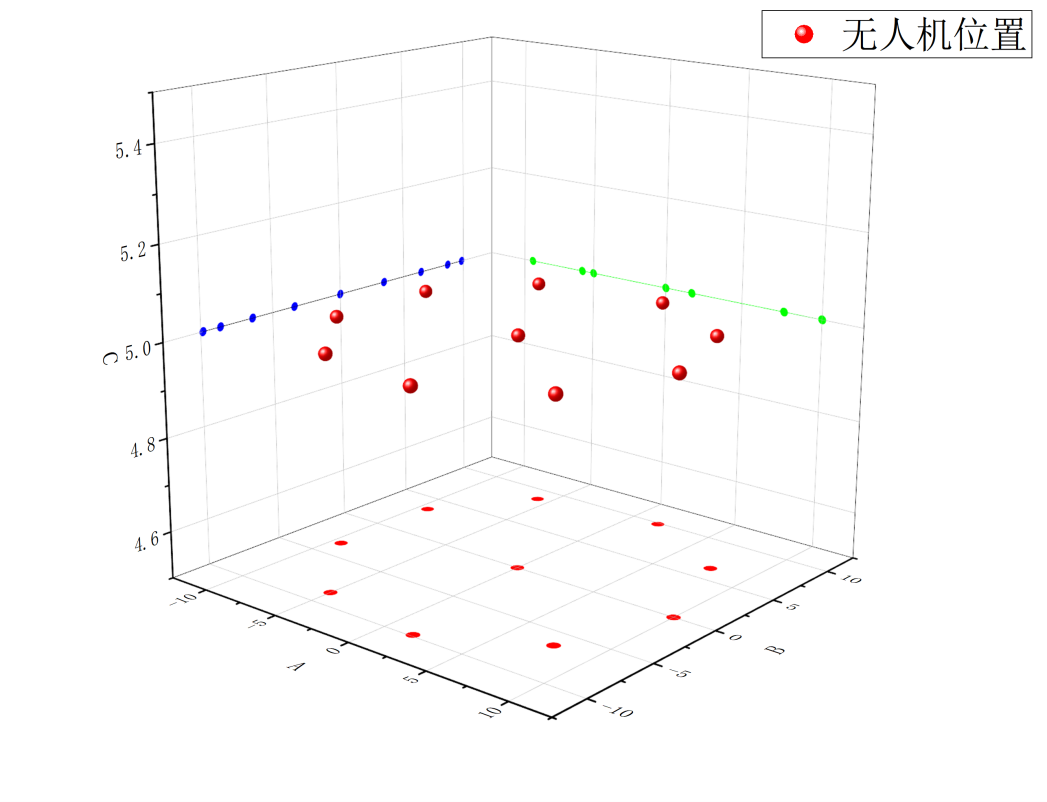
\includegraphics{res/PositionTheModelStereogram.png}
    \caption{检验定位模拟图}
\end{figure}


\subsection{问题1-2:求解实现有效定位的无人机数量}

\subsubsection{模型的分析}

为了方便后文描述,在此引入三圆定位模型的概念。

\begin{theorem}
    % \label{线段半径定理}
    在平面内,一线段两端(线段长度已知)和该线段垂直平分线上的一点所构成的角与该线段可构成圆及所得圆的半径。(本题以特殊角证明,但结论适用)
\end{theorem}

\begin{proof}
    设线段两端的端点为$a$和$b$,在线段$ab$垂直平分线上的点为$c$,连接线段$ac$和线段$bc$,分别做垂直平分线,相交于一点,此时可得一圆。设线段$ab$的长度为$l$,$\angle acb$的度数为$\alpha$。故有三角函数方程:

    \begin{equation}
        \frac{l}{\sin 2\alpha}=
        \frac{r}{\sin(\frac{\pi}{2}-\alpha)}
    \end{equation}

    解得

    \begin{equation}
        r=\frac{l}{2\sin\alpha}
    \end{equation}
\end{proof}

第二问基于第一问所建立的模型,已知某位置与理想模型位置存在偏差的无人机,接收到位置与理想模型位置无偏差且编号为 FY00和 FY01的无人机发射的信号,为实现位置偏差无人机的有效定位,还需一台或一台以上位置无偏差无人机发射信号。

\begin{figure}[h]
    \centering
    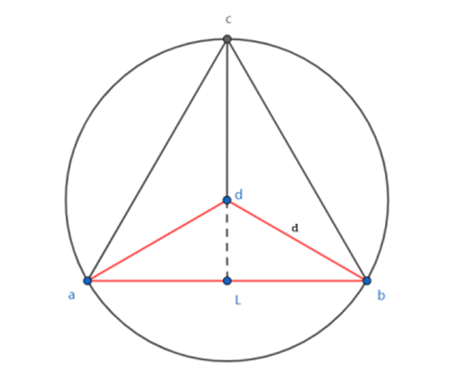
\includegraphics{res/lemmaFigure.png}
    \caption{引理图}
\end{figure}

\subsubsection{模型的求解}

如图。考虑到在直角坐标系下,求解圆形方程较繁琐,为简化计算,本小题在上一小题的基础上建立新的坐标系,使得无人机在同一平面内。设点$O$和点$A$分别是编号为$FY00$和$FY01$的无人机,它们的极坐标分别为点$O(0,0°)$和点$A(R,0°)$,点$P$是位置偏差的无人机且在线段$OA$的垂直平分线上,连接线段$OP$和$AP$,由引理确定圆$O_1$,设圆$O_1$的圆心为$O_1$,如图(为方便图解,此图为某理想状态,下文同)。最终编号未知无人机的偏离轨迹在劣弧$OO_1A$上。几何表示,设圆$O_1$的半径为$r_1$,则$r_1=\frac{R}{2\sin\alpha_1}$。

\begin{figure}[h]
    \centering
    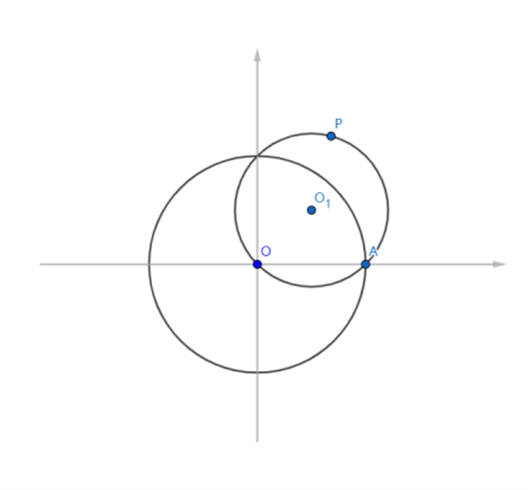
\includegraphics{res/figure102034.png}
    \caption{圆$O_1$位置简化图}
\end{figure}

即圆$O_1$的圆心坐标为:

\begin{equation*}
    \left(
        \frac{R}{2\tan\alpha_1},\frac{R}{2}
    \right)
\end{equation*}

即圆$O_1$的方程为:

\begin{equation}
    \left(
        x - \frac{R}{2\tan\alpha_1}
    \right)^2
    +
    \left(
        y - \frac{R}{2}
    \right)^2
    =
    \left(
        \frac{R}{2\sin\alpha_1}
    \right)^2
\end{equation}

另设一架发射信号无人机为点$B$,位置偏差无人机的位置为点$p_1$,连接$BP_1$、$OB$和$OP$,由引理确定圆$O_2$,设圆$O_2$的圆心为$O_2$。如图。即编号未知无人机的偏离轨道在劣弧$OO_2P_1$上。

\begin{figure}[h]
    \centering
    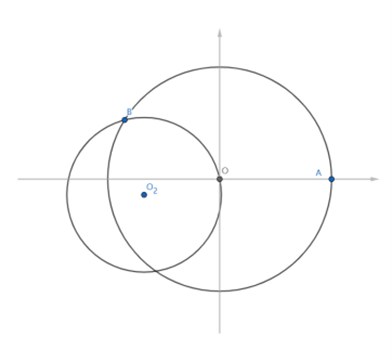
\includegraphics{res/figure04111100.png}
    \caption{圆$O_2$位置化简图}
\end{figure}

设圆$O_2$的半径为$r_2=\frac{R}{2\sin\alpha_2}$。

当圆$O_1$与圆$O_2$联立时,两圆相交于$O$点与另一点,此时除点外的交点就是偏差无人机的置。此时$B$点信号发射信号无人机位置及编号确定,与本题中除编号为FY00和FY01的无人机外,其他无人机位置及编号均未知的题意不符。依题意得,改变$B$点信号发射机的编号,即$B$点位置改变。此时,若不改变圆的半径,则两圆可能除点$O$外无交点;但倘若$B$点改变位置的同时,半径也随之改变,使之不管 点怎么改变,两圆都会相交于两个交点。这样即可确定$P$点无人机的位置,但与之而来的结果是 点可以出现在平面内绝大多数位置,即在实际操作中无法准确定位出接收信号无人机的位置。

\begin{figure}[h]
    \centering
    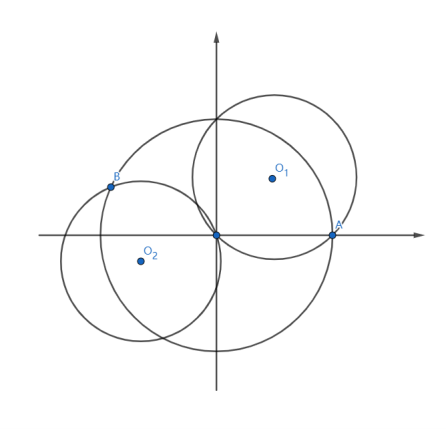
\includegraphics{res/figure111106.png}
    \caption{圆$O_1$、圆$O_2$联立图}
\end{figure}

证明有:设$B$点的坐标为$(x_1,y_1)$,当$B$点的横坐标$x$发生变化时,纵坐标$y$也随之变化,但由题易知$B$点坐标只有八个位置可以选择。设$A$点所占位置为第一个点(对无人机轨迹图做对称轴,$A$点在对称轴上)取值为$0$,设变量$a_2$为$\angle OO_1B$的角度大小,即$a_2$的取值范围为$\left[ 0,\pi \right]$,设变量$b_1$为轨迹图上$B$点所在位置的数值,即$b_1$的取值范围为$\left[ 1,8 \right]$。

\begin{equation}
    \begin{cases}
        x_1 = \cos(\frac{2\pi}{9}b_1 + \frac{\pi}{2}) \\
        y_1 = \sin(\frac{2\pi}{9}b_1 + \frac{\pi}{2}) \\
    \end{cases}
\end{equation}

 线段$BO$的斜率为:

 \begin{equation}
    k_1 = - \frac{x_1}{y_1}
 \end{equation}

 设圆心$O_2$到线段$BO$的距离为$\lambda_1$.

 由已知数据解得:

 \begin{equation}
    \lambda_1 = \frac{1}{2\tan\alpha_2}
 \end{equation}

 圆$O_2$的圆心坐标为:

 \begin{equation}
    \left(
        \frac{x_1}{2} + \lambda_1\cos(\arctan k_1),
        \frac{y_1}{2} + \lambda_1\sin(\arctan k_1)
    \right)
 \end{equation}

综上,圆$O_2$的表达式为:

\begin{equation}
    \left(
        x -
        \left(
            \frac{x_1}{2} + \lambda_1\cos(\arctan k_1)
        \right)
    \right)^2
    +
    \left(
        y -
        \left(
            \frac{y_1}{2} + \lambda_1\sin(\arctan k_1)
        \right)
    \right)^2
    =
    \left(
        \frac{R}{2\sin\alpha_2}
    \right)
\end{equation}

联立方程,得出除了$(0, 0)$外的无数个解,不符合实际。

\begin{figure}
    \centering
    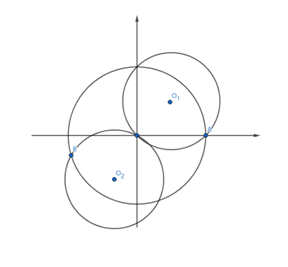
\includegraphics{res/figure111121.png}
    \caption{两圆位置关系示意图}
\end{figure}

对此,再设一架发射信号无人机为点$C$,位置偏差无人机的位置为点$P_2$,连接$OP_2$、$OC$和$CP_2$,由引理确定圆$O_3$,如图。同上理得编号未知无人机的偏离轨道在劣弧上。几何表示有:

\begin{figure}
    \centering
    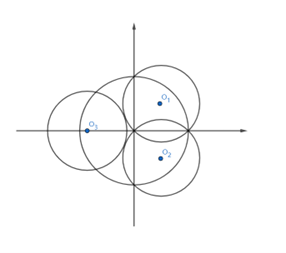
\includegraphics{res/figure111123.png}
    \caption{三圆联立图}
\end{figure}

设圆$O_3$的半径为$r_3$,则$r_3=\frac{R}{2\sin\alpha_3}$。此时在坐标平面内除轨迹圆外还有三个圆。由前文假设,得出相应结论,即圆$O_3$的数据为:变量$a_3$,$C$点坐标为:

\begin{equation}
    \begin{cases}
        x_2 = \cos\left(
            \frac{2\pi}{9}b_2 + \frac{\pi}{2}
        \right) \\
        y_2 = \sin\left(
            \frac{2\pi}{9}b_2 + \frac{\pi}{2}
        \right)
    \end{cases}
\end{equation}

线段$OC$斜率:

\begin{equation}
    k_2 = - \frac{x_2}{y_2}
\end{equation}

圆点$O_3$到线段$OC$的距离为:

\begin{equation}
    \lambda_2 = \frac{1}{2\tan\alpha_3}
\end{equation}

圆心$O_3$的坐标:

\begin{equation}
    \left(
        \frac{x_2}{2} + \lambda_2\cos(\arctan k_2),
        \frac{y_2}{2} + \lambda_2\sin(\arctan k_2)
    \right)
\end{equation}

圆$O_3$的表达式:

\begin{equation}
    \left(
        x -
        \left(
            \frac{x_2}{2} + \lambda_2\cos(\arctan k_2)
        \right)
    \right)^2
    +
    \left(
        y -
        \left(
            \frac{y_2}{2} + \lambda_1\sin(\arctan k_2)
        \right)
    \right)^2
    =
    \left(
        \frac{R}{2\sin\alpha_3}
    \right)
\end{equation}

为方便后续计算,在此对圆$O_1$添加一个变量$a_1$,使得圆$O_1$大小可改变。改变$b_1$和$b_2$的大小,此时两个圆开始移动;与此同时改变$a_1$、$a_2$和$a_3$的大小,让圆$O_1$、圆$O_2$和圆$O_3$大小改变。当三圆相交于两交点时,便确定$P$点位置,从而确定偏无人机的位置。

\begin{figure}
    \centering
    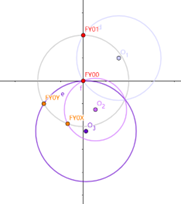
\includegraphics{res/figure111138.png}
    \caption{三圆定点模型示意图}
\end{figure}

综上所述,求得模型方程组为:

\begin{equation}
    \begin{cases}
        \left(x - \frac{R}{2\tan\alpha_1}\right)^2 +
        \left(y - \frac{R}{2}\right)^2 =
        \left(\frac{R}{2\sin\alpha_1}\right)^2    \\

        \left[x - (\frac{x_1}{2} + \lambda_1\cos(\arctan k_1))\right]^2 +
        \left[y - (\frac{y_1}{2} + \lambda_1\sin(\arctan k_1))\right]^2 =
        \left(\frac{R}{2\sin\alpha_2}\right)^2    \\

        \left[x - (\frac{x_2}{2} + \lambda_2\cos(\arctan k_2))\right]^2 +
        \left[y - (\frac{y_2}{2} + \lambda_21\sin(\arctan k_2))\right]^2 =
        \left(\frac{R}{2\sin\alpha_3}\right)^2    \\
    \end{cases}
\end{equation}

从而确定还需两架发射信号无人机才能确定位置偏差无人机的定位。

% \fbox{
% \begin{minipage}[h]{30em}
%     \centering
%     \begin{enumerate}
%         \item 第一次调整由FY00、FY03、FY06、FY09四架无人机发射信号,其余无人机接收信号并且调整自己的位置
%         \item 以其中某个接收信号的无人机为研究对象,记该无人机为A
%         \item 无人机A接收到三个方向信号,根据三圆定位模型计算出自己的位置P1
%         \item 无人记A根据自己的编号计算出自己的理想位置P2
%         \item 无人记A根据前两部计算出的P1、P2计算出位置修正向量j1
%         \item 无人记A根据修正向量调整自己的位置
%         \item 所有无人机执行上述步骤后,将全部位于同一圆周上
%         \item 第二次调整由FY00、FY01两架无人机发射信号,其余无人机接收信号并且调整自己的位置
%         \item 以其中某个接收信号无人机为研究对象,记该无人机为B
%         \item 无人机B接收到一个方向信息,根据该信息计算出自己的位置P3
%         \item 无人记B根据自己的编号计算出自己的理想位置P4
%         \item 无人记B根据前两部计算出的P3、P4计算出位置修正向量j2
%         \item 无人记B根据修正向量j2调整自己的位置
%         \item 所有无人机执行上述步骤后,将全部均匀的分布在圆周上
%     \end{enumerate}
% \end{minipage}
% }

\subsection{问题1-3:由已知条件及表1数据给出相应的调整方案}

在该小节中,首先引入下面的引理:

\begin{theorem}
    在极坐标系钟,已知$A(\rho_1, \theta_1)$、$B(\rho_2, \theta_2)$,则平面直角坐标系钟的$\widehat{AB}=(\rho_2\cos\theta_2 - \rho_1\cos\theta_1, \rho_2\sin\theta_2 - \rho_1\sin\theta_1)$.
\end{theorem}

\begin{proof}
    以点$O$为圆心,极坐标$\rho$轴正方向为$x$轴正方向。则根据参数方程:

    \begin{equation*}
        \begin{cases}
            x = \rho\cos\theta\\
            y = \rho\sin\theta\\
        \end{cases}
    \end{equation*}

    则设$\overrightarrow{OA}$为$(\rho_1\cos\theta_1, \rho_1\sin\rho_1)$,$\overrightarrow{OB}$为$(\rho_2\cos\theta_2, \rho_2\sin\rho_2)$,故有

    \begin{equation}
        \begin{aligned}
            \overrightarrow{AB} &= \overrightarrow{OB} - \overrightarrow{OA} \\
            &=(\rho_2\cos\theta_2 - \rho_1\cos\theta_1, \rho_2\sin\theta_2 - \rho_1\sin\theta_1)
        \end{aligned}
    \end{equation}
\end{proof}

为了使$1$架无人机位于圆心位置,其余$9$架无人机均匀的分布在某个圆周上,可进行下来两次调整。

第一次调整时,圆心上的FY00无人机和圆周上的FY03、FY06、FY09三架飞机遂行发射信号,其他无人机接收这四架无人机的信号,每个无人机都可获得三个方向信息。

以其中某架无人机为研究对象,记该无人机为点$Q$,设其获得角度信息为$\alpha_1$、$\alpha_2$、$\alpha_3$。此时,于点$Q$而言,圆周上的三架发射信号无人机的位置不确定,为了方便后文分析,不妨令其中一架发射信号无人机所在方向为极坐标正方向,建立极坐标系。那么另外两架无人机必然分布在同一圆周上。





\section{模型评价与推广}

\subsection{模型优点:}

\begin{itemize}
    \item 三圆定位模型的引理选取合理,以坐标系为基础改变偏差轨迹圆的数值,侧面验证了三圆定位模型的合理性,避免了单个圆的各方面数据计算,减少了运算量。\cite{TongJiDaXueShuXueXiGaoDengShuXue}
    \item 对无人机定位上运用到定位模型,让无人机位置出现在三维或二位空间,让模型在处理时更加灵动化,科学合理的预估出偏离无人机的大概位置。
    \item 本文运用到定位模型及一些主观构思,即能减少主观构思的不足,又能与实际结合,具有一定的科学性和适用性。
    \item 运用一些特殊算法和特殊坐标系,误差很小,具体的论证的本文的科学性,有一定的参考价值。
    \item 通过合理的假设,并保证模型计算结果精确性的条件下,有效降低了计算结果的复杂程度
\end{itemize}

\subsection{模型缺点:}

\begin{itemize}
    \item 引入的引理和三圆定位模型具有一定的主管构想,数据处理上有一定的局限性,处理实际问题时存在偏差。
    \item 本文约束条件较多,实际操作上处理无源定位还和众多因数有关。例如:空气阻力及无人机自身重力。
\end{itemize}

\subsection{模型的推广:}

在大数据的背景下,根据本文对无源定位的模型计算一定程度上便捷了相关工作人员。同样,本文在计算的同时也参杂了一些合理的主观构想和特殊数据,在合理的同时也具有一定的不确定性。
